\documentclass{sigchi}

\toappear{}
\pagenumbering{arabic}

% Load basic packages
\usepackage{balance}
\usepackage{graphics}
\usepackage[T1]{fontenc}
\usepackage{txfonts}
\usepackage{times}
\usepackage{url}
\usepackage{color}
\usepackage{textcomp}
\usepackage{booktabs}
\usepackage{ccicons}
\usepackage{todonotes}
\usepackage[pdftex]{hyperref}

% llt: Define a global style for URLs, rather that the default one
\makeatletter
\def\url@leostyle{%
  \@ifundefined{selectfont}{\def\UrlFont{\sf}}{\def\UrlFont{\small\bf\ttfamily}}}
\makeatother
\urlstyle{leo}

% To make various LaTeX processors do the right thing with page size.
\def\pprw{8.5in}
\def\pprh{11in}
\special{papersize=\pprw,\pprh}
\setlength{\paperwidth}{\pprw}
\setlength{\paperheight}{\pprh}
\setlength{\pdfpagewidth}{\pprw}
\setlength{\pdfpageheight}{\pprh}

% Make sure hyperref comes last of your loaded packages, to give it a
% fighting chance of not being over-written, since its job is to
% redefine many LaTeX commands.
\definecolor{linkColor}{RGB}{6,125,233}
\hypersetup{%
  pdftitle={SIGCHI Conference Proceedings Format},
  pdfauthor={LaTeX},
  pdfkeywords={SIGCHI, proceedings, archival format},
  bookmarksnumbered,
  pdfstartview={FitH},
  colorlinks,
  citecolor=black,
  filecolor=black,
  linkcolor=black,
  urlcolor=linkColor,
  breaklinks=true,
}

% create a shortcut to typeset table headings
% \newcommand\tabhead[1]{\small\textbf{#1}}

% End of preamble. Here it comes the document.
\begin{document}

\title{An Interactive Visual Analytics Dashboard for the Employment Situation Report}

% \numberofauthors{4}
% \author{%
%   \alignauthor{Benjamin Bengfort\\
%     \affaddr{University of Maryland}\\
%     \email{bengfort@cs.umd.edu}}\\
%   \alignauthor{Xintong Han\\
%     \affaddr{University of Maryland}\\
%     \email{hixintonghan@gmail.com}}\\
%   \alignauthor{Assaf Magen\\
%     \affaddr{University of Maryland}\\
%     \email{amagen@umd.edu}}\\
%   \alignauthor{Hao Zhou\\
%     \affaddr{University of Maryland}\\
%     \email{zhhoper@gmail.com}}\\
% }

\numberofauthors{1}
\author{%
    \alignauthor{Benjamin Bengfort, Xintong Han, Assaf Magen, and Hao Zhou\\
        \affaddr{Department of Computer Science, University of Maryland}\\
        \email{\texttt{\{bengfort,xintong,amagen,hzhou\}@cs.umd.edu}}\\
    }\\
}

\maketitle

\begin{abstract}
The \textit{Employment Situation Report} is a monthly news release by the Bureau of Labor Statistics which describes the results of the Current Population Survey \cite{_employment_2015}. Its release is widely anticipated by economists, journalists, and politicians as it is used to forecast the economic condition of the United States by describing ongoing trends and has a broad impact on public and corporate economic confidence leading directly to investment decisions. The report itself is in a PDF format that is comprised primarily of text and tabular information. Quickly and correctly interpreting the results of the jobs report is vital for quality reporting and decision making, but the report is more suited for longer study than deriving insights. In this project we explore the use of an interactive dashboard for visual analytics upon the released BLS data. Using an application demonstration and a usability study we will show that visually interacting with the most current employment data, users are able to rapidly achieve rich insights similar to those reported on in the text of the Employment Situation Report.
\end{abstract}

\keywords{
	Employment Situation Report; Information Visualization; Visual Analytics; Dashboard; D3; Data Science Pipeline
}


\section{Introduction}
The \textit{Employment Situation Report} is a critical, monthly assessment of the state of labor in the United States which is released by the Bureau of Labor Statistics (BLS) at 8:30 AM on the first Friday of the month. The ``Jobs Report'', as it's popularly called, is based on the Current Population Survey, which surveys individual households and the Current Employment Statistics Survey, which surveys employers. Together, these two surveys give a snapshot view of the number of employed and unemployed Americans, how many hours they are working, and a variety of other facts and figures. In recent years, this report has been used to measure economic and political solutions to the 2008 downturn, as well as the performance of politicians themselves. As a result, news media widely publicizes the upcoming release of the report each month, then follows the publication with widespread analyses and critiques. Perhaps thanks to its publicity the report is more recently being used as a forecasting tool by firms on Wall Street because the report is an indicator of investor and employer confidence in the growth of the economy since more jobs mean more consumer spending \cite{mahorney_what_2013}.

The report is delivered in both PDF and HTML format, comprised mostly of text and tabular information and is well suited to deep study rather than rapid analysis. Because of the report's forecasting power and journalistic impact, fast and correct interpretation of the report's information is essential; however, the current format does not lend itself well to the quick derivation of insights. Moreover, the report is not as easily accessible to a general audience, favoring economic language and measurements. We believe that a \textit{visual analytics} methodology \cite{keim_mastering_2010} using information visualization techniques would benefit the \textit{Employment Situation Report}, allowing for fast, correct interpretation of the current employment situation in the United States, as well as making the report more generally accessible.

The combination of computer analytical processes with the human ability to quickly understand patterns leads to a reasoning system of discovery through interaction \cite{green_visual_2008}. Computer systems that enhance a user's sense-making process of ``overview first, zoom and filter, and details on demand'' allow the fast formulation and verification of hypothesis and will often lead to richer, deeper insights than can be extracted simply through statistical techniques \cite{heer_interactive_2012}. Importantly, few prerequisites are required for these types of analyses as essential domain knowledge can be incorporated into the analytical framework, leading to accessibility beyond those traditionally required for research. By creating a visual analytical system that adheres to these requirements, the Jobs Report will be made more widely available and reporting on the employment situation more verifiable.

In this project, we explore the development of an interactive ``Employment Report Dashboard'' web application (nicknamed ELMR), which implements a variety of visual tools for the exploration of the vast amount of time series data generated by BLS surveys. ELMR combines data from national surveys as released in the \textit{Employment Situation Report} as well as geographic-specific surveys that deal with state and metropolitan populations. Through interactive exploration with the tools on the application, users are able to explore both current and historical contexts for the employment situation and rapidly develop and verify hypotheses that could lead to important insights.

\begin{figure*}[!ht]
  \centering
  \includegraphics[width=1.6\columnwidth]{figures/dashboard.png}
  \caption{The ELMR application focuses on interactive visual analyses of employment data at both the national and state level. This screen grab shows the primary dashboard for time series exploration, as well as the tabs for selecting other visual analyses.}~\label{fig:dashboard}
\end{figure*}

The rest of the paper is structured as follows. We will first describe the ingestion framework required for dealing with BLS data and preparing a web application that must be updated on a monthly basis. We will then describe the four dashboards that we have implemented for visual exploration: a Time Series Explorer, a Geography Choropleth, a four dimensional ``Wealth of Nations'' visualization, and data exporter. We will evaluate the utility of our tool for visual analytics on the employment situation report via a usability study, and finally will conclude with a discussion including related and future work.

\section{The BLS Data Pipeline}

The Jobs Report is released monthly based primarily on two national surveys: the Current Population Survey and the Current Employment Statistics survey. In order to achieve a ``dashboard of visualizations'', described in the section on design and as shown in Figure~\ref{fig:dashboard}, we also ingested data from state and metropolitan surveys: the Local Area Unemployment Statics survey and Current Employment Statistics for State and Metropolitan economic divisions. Using these data sources created a unique challenge for a visual analytics data product - the system had to be able to adapt and acquire new information automatically, and to display important headlines on demand.

Our initial architecture therefore relied on the pedagogical model of the ``data science pipeline'' as described in \cite{ojeda_practical_2014}. The data science pipeline is an analytical framework, describing preparatory analytical steps of ingestion, wrangling, storage, and pre-computation. We replaced inferential and modeling statistical methodologies with a visual analysis methodology. The resulting ``BLS Data Pipeline'' is described by Figure~\ref{fig:pipline}. The ingestion component utilized the BLS API to download individual time series, which then had to be wrangled to normalize the data and impute missing values for storage. Initial computations were then run on the data set to generate other data sources (for example a rate of change data set was computed on each time series). The data storage then powered an interactive API that was utilized by our visual front-end.

\begin{figure}[!h]
    \centering
    \includegraphics[width=0.9\columnwidth]{figures/pipeline.png}
    \caption{The BLS data pipeline, a model for combining monthly data ingestion with a visual analytics workflow.}~\label{fig:pipline}
\end{figure}

In this section we will briefly cover the data sources used in our project, as well as the associated architecture of our implementation.

\subsection{Data Sources}

The Bureau of Labor Statistics provides a large amount of data gathered by surveys conducted by various organizations of the United States Department of Labor. Three independent surveys: the Current Population Survey, the Current Employment Statistics survey, and the Local Area Unemployment Statistics survey provide the majority of information that is used in our application to explore the employment situation of the United States at both the national and state levels. Each of these data sources adds dimensions to a variety of visual analyses, and when contextualized together provides the best possible opportunity for insight discovery.

The primary data source for the Jobs Report is the Current Population Survey (CPS) \cite{_labor_????}, which is a monthly survey of households. This survey focuses on the relationship between demographics and employment and at the national scale provides a comprehensive data set on the labor force, unemployment, earnings, hours of work, and other labor characteristics. It is in this survey that demographic statistics like gender, age, education level, or ethnicity are gathered.

A secondary source for the Jobs report, the Current Employment Statistics survey (CES) surveys employers rather than households for labor force information \cite{_current_2015}. The CES survey is not only national, but also provides granular data for state and metropolitan geographies as well. In our application we diffrentiate between national and local CES surveys with the acronyms CES and CESSM respectively. This survey focuses on industry-specific details of employment, hours, payroll, and earnings and is useful as a classification for different labor categories rather than demographics.

Finally, the Local Area Unemployment Statistics survey (LAUS) fills in local regional information that relates demographic information to employment where the CPS only describes the national level \cite{_local_2015}. LAUS provides monthly employment, unemployment, and labor force data by census divisions that include states, counties, metropolitan areas, and many cities. Because LAUS is a household survey (by place of residence) the employment characteristics can give a much more focus view of how demographic trends influence employment and the local level.

All of these data sets can be affected by seasonal events which follow a regular pattern which will influence employment statistics. For example, each June a large number of youth enters the labor force, which could obscure other less structural trends and changes for may. In order to minimize the impact of seasonality, most of these data sets are adjusted for seasonality. Finally, datasets can be grouped by a variety of dimensions. The employment dimensions include ``employment'', ``unemployment'', ``unemployment rate'', and ``labor force''. CES dimensions included industry descriptions like ``Mining and Construction'', whereas CPS and LAUS focused on demographic dimensions like age, gender, ethnicity, or level of education. Geographic dimensions had to be included for the CESSM and LAUS data sets, ordered by both U.S. Census economic divisions as well as by state.

\subsection{Data Ingestion}

The Bureau of Labor statistics provides two public data APIs that use RESTful state transfer mechanisms to deliver data on demand to the user for particular time series information in various BLS programs. The APIs accept HTTP requests for information to URL endpoints that describe the required resource, then return information in paginated JSON format. We used the Version 2.0 implementation of the BLS API, which requires registration to obtain an API key. Such registration allows BLS to better understand what applications are using its data, but also allows developers more flexible access to the BLS data source.

We created a general Python tool for downloading BLS data by providing a list of BLS IDs for time series. There are three primary ways of ingesting time series: by downloading a single source or multiple sources to an endpoint that only allows downloading of data for the past three years, or by using the registration endpoint to specify the start and end years for ingesting multiple time series. We ingested data for the current millennium: from January, 2000 to February, 2015, obtaining over 305,445 records from 1,684 time series. To obtain a list of time series to target our downloads, we wrote a web scraper which scraped the ``most popular'' pages from the BLS website itself.

\subsection{Data Wrangling and Storage}

Data from the BLS website is returned in a JSON form, however each data source from individual surveys may be formulated differently. Data wrangling efforts primarily dealt with imputing missing data (from years where surveys were not collected) and correcting mistakes in the ingestion process (e.g. mislabeling series information). Data type conversion was also required as JSON is a string format. The result of the wrangling process was a normalized, relational data set that could be stored in a PostgreSQL database management system.

The data wrangling system also computed ``extra'' data sources that we thought might be interesting to the front end visualization. One of the primary extra sources was to compute the ``percent rate of change'' which computed the percent delta from one time period to the next. We utilized the formula $r_i = \frac{r_i - r_{i-1}}{r_i} + \epsilon \times r_{i-1}$ to compute the rate of change, which was regularized by some parameter, $\epsilon$, which we initially set to $0.01$.  It was our hope that by including pre-computed data sets such as these, the visual exploration mechanism could combine both human and computer analytical efforts.

\begin{figure*}[!ht]
    \centering
    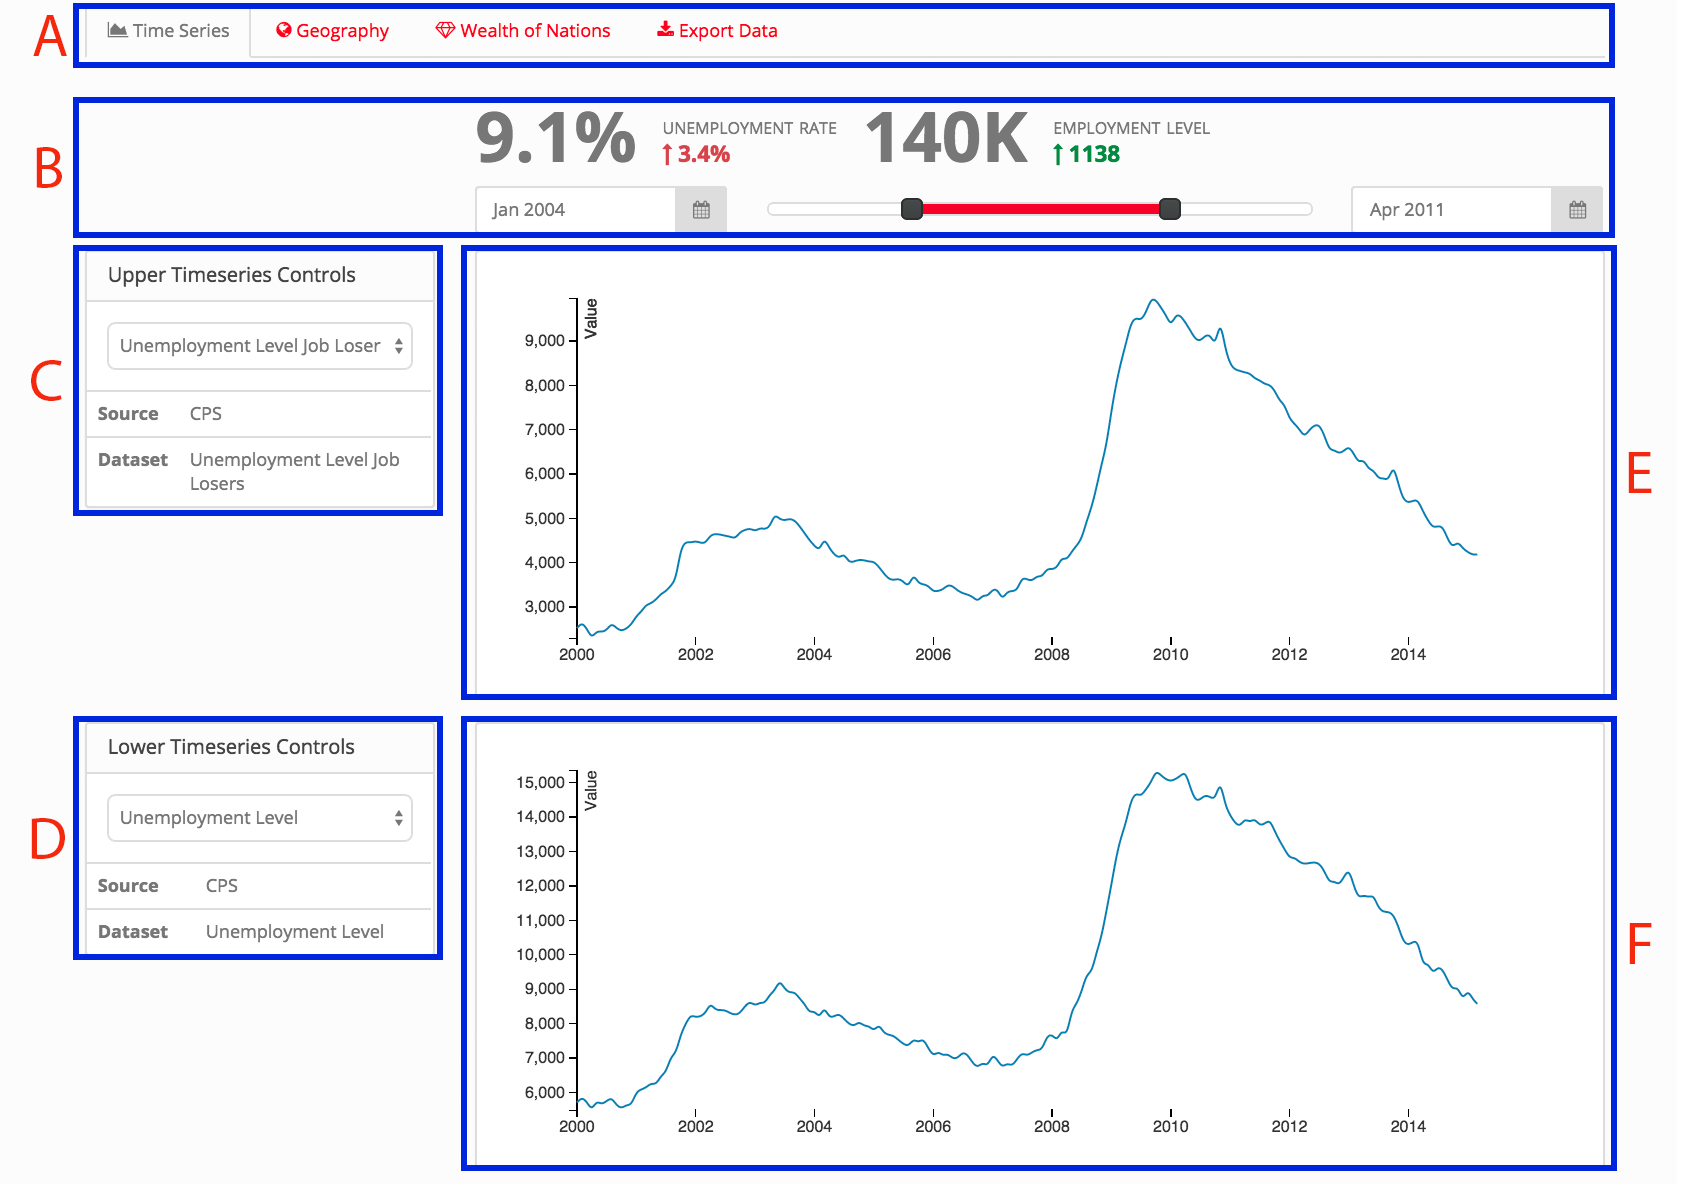
\includegraphics[width=1.75\columnwidth]{figures/time_series_new_1.png}
    \caption{The time series explorer dashboard allows the user to visualize multiple raw time series information in two different charts for ease of comparison with different data ranges. The year slider allows zooming and filtering by year. Finally, this dashboard attempts to add important headlines as listed by the Jobs Report.}
    \label{fig:time_series}
\end{figure*}


Data wrangling also involved our initial data exploration efforts. We discovered that in order to power our geographic analyses, we needed some sort of regional information (e.g. FIPS identification codes or larger economic areas). The BLS website, while providing information particularly related to a time series, provided no \textit{meta information} about the data source, which required other data sources. For example, although we might download a time series entitled ``Tennessee, Professional and Business Services, Not seasonally adjusted - labor force'' - we still had to do the work of assigning the Tennessee FIPS code, 42, and to parse out whether or not the data set was seasonally adjusted, what dataset it related to (labor force) and what its modifier was (Professional and Business Services). To do this for 1684 data sources, we needed an automated mechanism to parse time series names. The challenges of adapting the data straight from the BLS website took up over 80\% of our development effort, and perhaps highlight how vital a visual analysis tools is to augment straight data flow.

\subsection{System Architecture}

The ingestion mechanism can be polled on a monthly basis to retrieve new information from the BLS API, keeping the application up to date for immediate use by journalists. The data backend then powers a RESTful API built using Python and the Flask framework that serves a front-end javascript single page application, which primarily uses D3 for visualization methodologies. Other notable implementation details can be found on the Github project page: \url{https://github.com/bbengfort/jobs-report/}, where we have made our system open source using the MIT license. The ELMR project itself is currently deployed on Heroku and can be accessed via \url{http://elmr.herokuapp.com/}. It is our intent that this project can be explored in detail by the scientific and data community.

\section{ELMR Design}

The data provided by BLS that powered our web application came in the form of time series data. Although each individual time series did not contain massive amounts of information (approximately 182 data points representing each month in this millenium), the number of time series themselves exceed the ability for a human to organize and digest the various information. In order to provide a visual mechanism of exploration and interactive reasoning our design philosophy was that of a ``dashboard of visualizations'' where users could select appropriate visualizations, and interact with them though the ``overview first, zoom and filter, details on demand'' sense-making process. The primary filtering process involved time sliders to create windows of time to explore, as well as selectively choose which data to include in the visualizations.

We implemented four dashboards to explore these techniques, each in their own seperate tabs across the top of the application:

\begin{enumerate}
    \item \textbf{Time Series Explorer}: explore and compare specific time series data sets in a dual-graph display.
    \item \textbf{Geographic Choropleth}: explore time series according to their regional factors and influences, and how regions change over time.
    \item \textbf{Wealth of Nations}: inspired by a classic visualization, this is a four dimensional analysis of regional data.
    \item \textbf{Data Export Utility}: other visualization tools might benefit from the ingestion and wrangling work we've undertaken, data export allows you to use the data in your tool of choice.
\end{enumerate}

The visual analytical process requires a ``dashboard'' methodology - where a user can interactively control as many aspects of the visualization as possible, and where multiple visualizations are adapted simultaneously. Each tab described above is a dashboard with its own custom controls. The Time Series Explorer allows users to explore all of the time series with two chart windows and filter and zoom by a range of years. This explorer also has a ``headline view'' which attempts to highlight key information. The Geography Choropleth allows the user to explore regional information in the continental United States, while also filtering for percent change. The ``Wealth of Nations'' attempts to minimize the affect of the geographic size on analytical ability from the Choropleth maps and is based on a classic visualization made famous by Hans Rosling's 2006 TED Talk \cite{_wealth_????}. Finally, a data export dashboard allows the user to download specific data with filters applied so that they can manipulate the data in their favorite visualization tools.

\subsection{Time Series Explorer}

Figure~\ref{fig:time_series} shows our design of time series dashboard. The primary focus of this dashboard are two, stacked time series graphs, which allow for multiple visual analysis of time series with different $Y$ dimensions or scales, but with the same $X$ dimension - that is the period of the time series. In order to better describe the dashboard, we have divided it into six regions labeled A-F, which we will describe in detail below.

Region A shows four tab navigation bars which allow the user to switch between the four implemented dashboards. The tab display is consistent across all dashboards, and as more visualizations are added to the ELMR interactive visual analysis tool, more tabs can be added as well. If the list of tabs grows too long, in the future we intend to allow the user to select tabs for a personalized display that gives them quick access to the dashboards they use most (for example, national reporters may be less interested in local employment statistics).

Region B contains an ``at-a-glance headline view'' and year slider control. The headline view is intended to be an eye-catching ``at-a-glance'' instant insight framework that is based heavily on the headline in the Employment Situation Report. The headline is tied to the two major pieces of information that are published at the top of the report - the unemployment rate and the number of non-farm jobs. The at-a-glance headline also displays important information regarding the amount of \textit{change} from the last period - a major piece of information that most users want to know right off the bat. It is for this reason that these headlines have such a prominent place in our application.

The year slider control also shown in Region B is one of the primary mechanisms for zooming and filtering information for every dashboard in the app. The year range slider allows the user to select a window of time periods within the analytical time span, to zoom the data into that range. Other dashboards have period selectors rather than ranges, which allows the user to identify trends or data for a specific period.

Regions C and D contain the primary controls for the time series displays in regions E and F respectively. There are many BLS Time Series, for this application we have downloaded 1684 data sets, each of which can be displayed. The challenge is how to allow a user to select data sets of interest quickly. Although we toyed with using an autocomplete or search mechanism, our prototype implementation simply uses a grouped, auto complete dropdown as shown in Figure~\ref{fig:select}. This design follows ``prevent error'' rule in the Eight Golden Rules of User Interface Design \cite{shneiderman_eight_????} as the user can only select the databases that are available through our drag-down menu.

\begin{figure}[h]
    \centering
    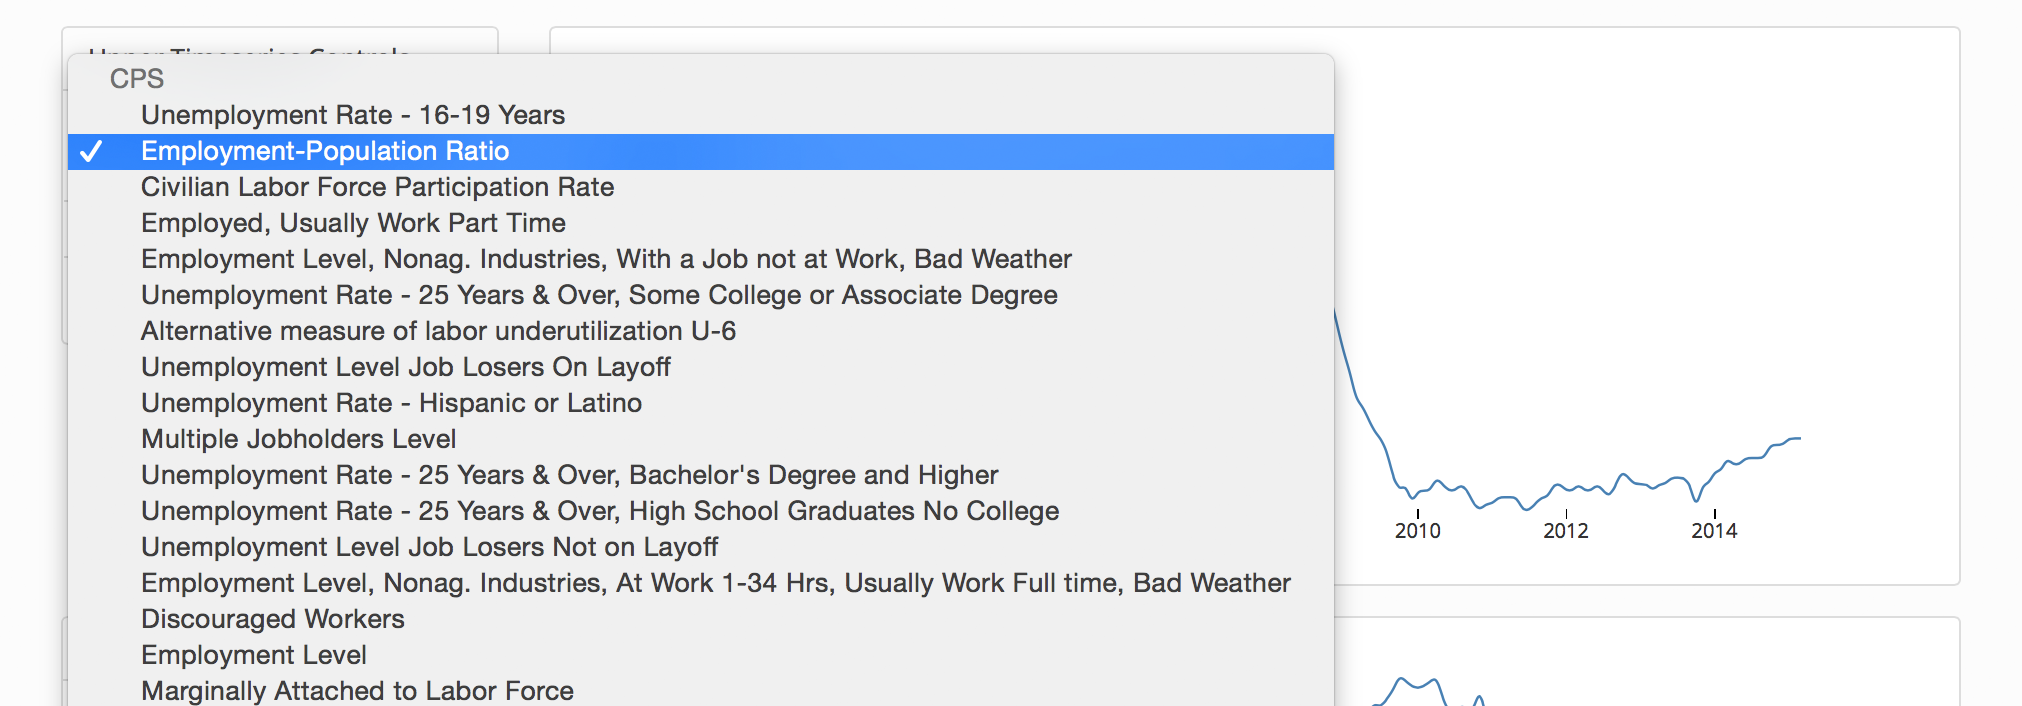
\includegraphics[width=0.9\columnwidth]{figures/select.png}
    \caption{In order to minimize error, users select BLS time series data sets through a grouped, alphabetized dropdown.}
    \label{fig:select}
\end{figure}

Region E and F are used to show two time series graphs. The graphs shown in region D and E correspond to the  database selected in region B and C respectively.

\subsection{Geography Choropleth}

\begin{figure*}[!ht]
    \centering
    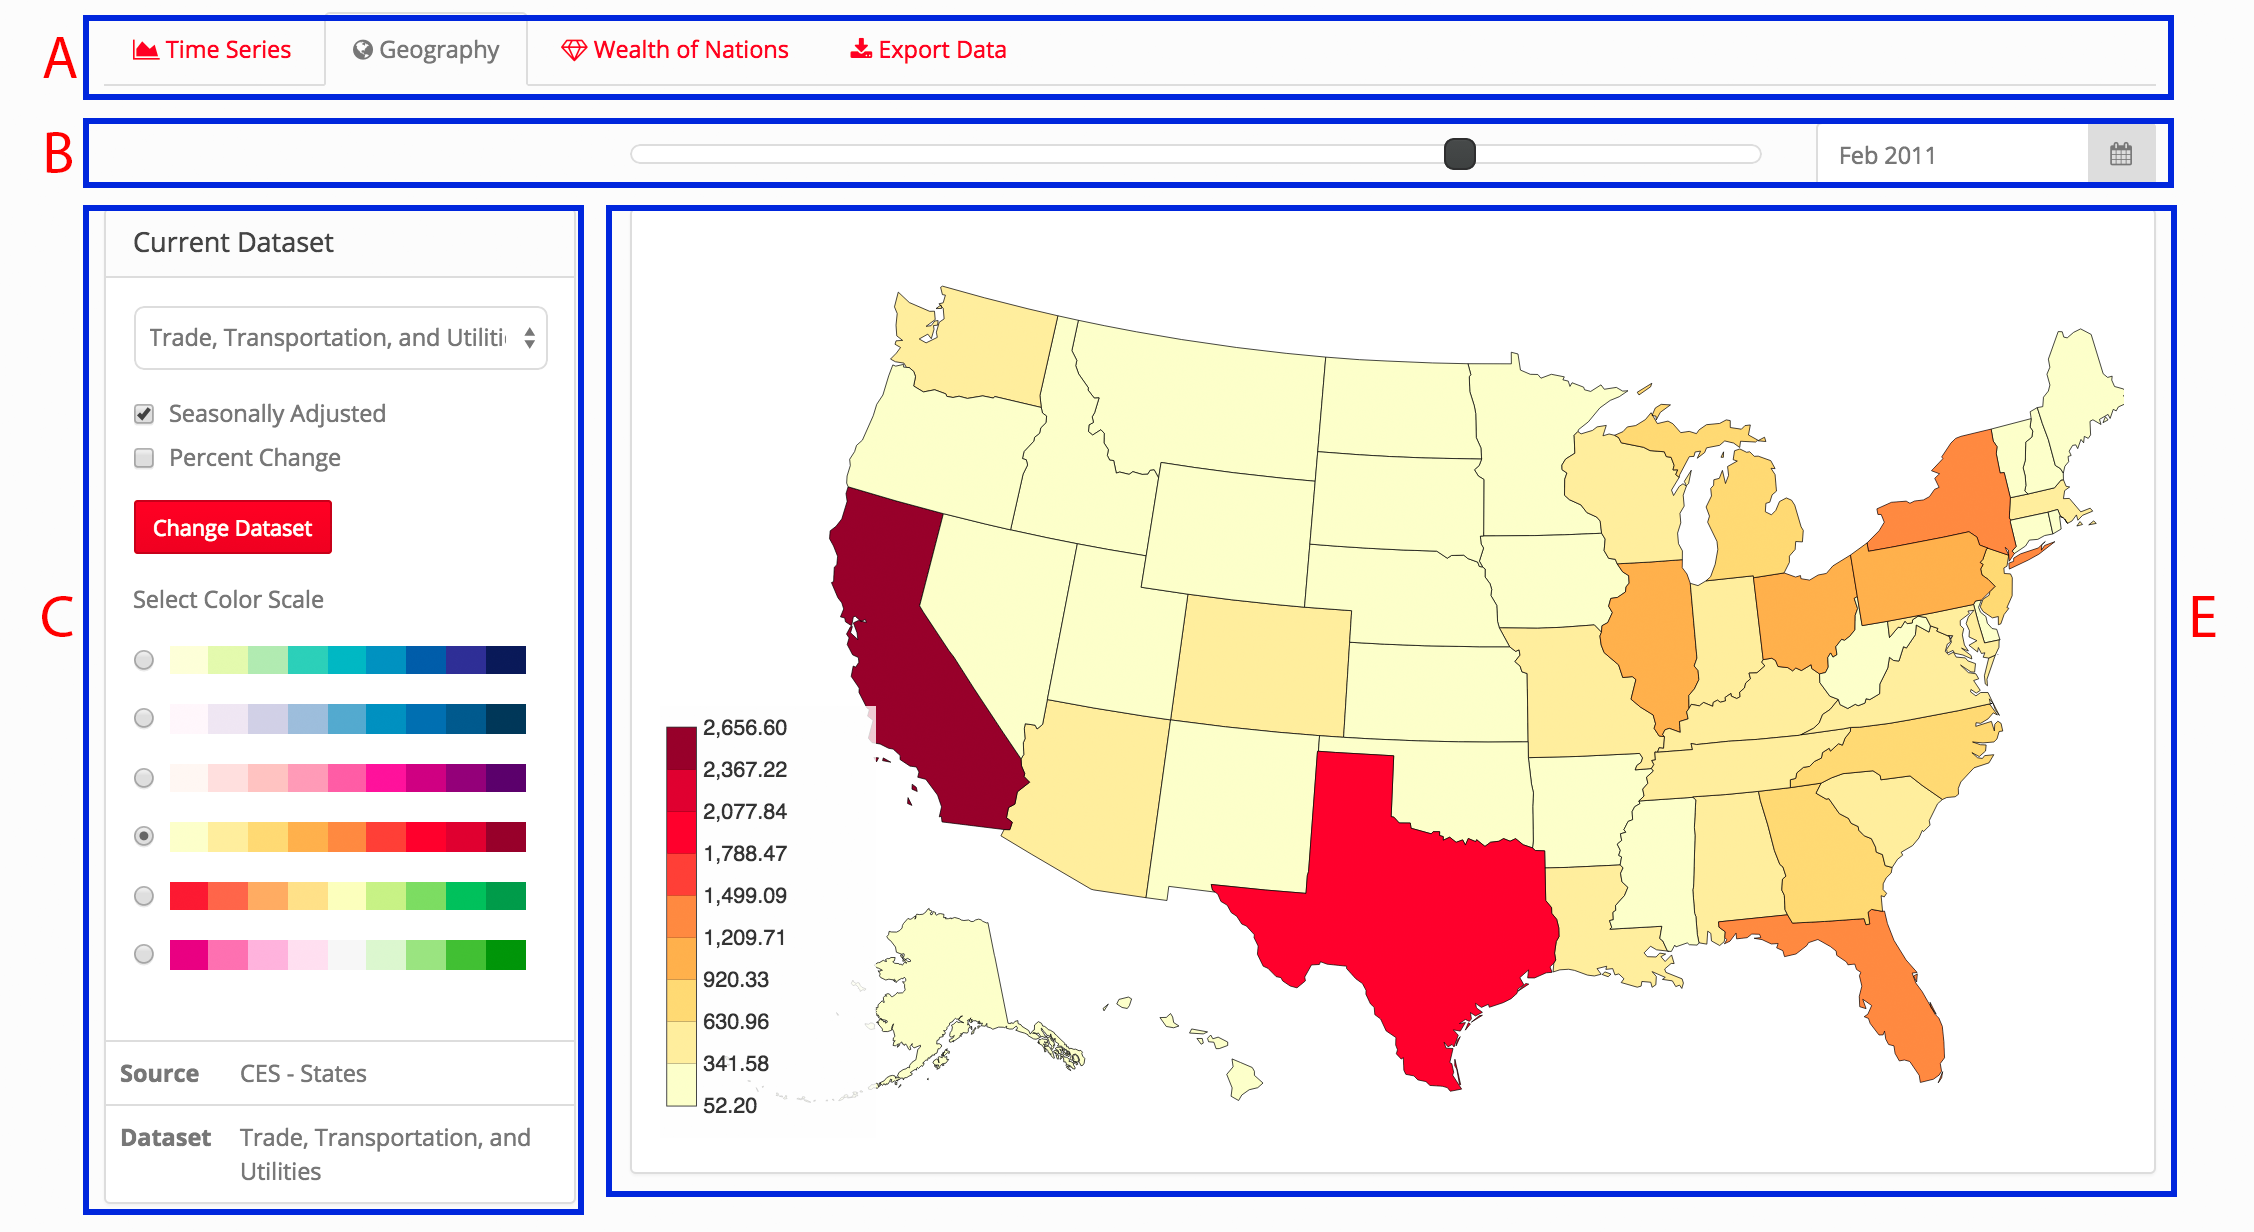
\includegraphics[width=1.75\columnwidth]{figures/geography_new_1.png}
    \caption{The Geography Choropleth dashboard implements a chorpleth style heatmap on the AlbersUSA projection of the United States, particularly at the state and regional level. Users can control the data set and colors with the control bar, and select the time period to visualize with a slider.}
    \label{fig:Geography}
\end{figure*}

Our second visual dashboard focused particularly on regional or state visual analyses by implementing a highly interactive choropleth map of the United States using the AlbersUSA projection, as shown in Figure~\ref{fig:Geography}. The dominant feature of this dashboard is the choropleth map of the United States which is directly connected to a selectable dataset from either the CESSM or LAUS datasets. By interacting with the controls on the left, users can set the data set, whether or not to implement seasonal adjustments, select the rate of change dataset, and even select the color map. A slider at the top of the visualization controls the year for the map.

This style map was our first design for the application, and we focused heavily on its implementation. However, we discovered that the datasets were heavily weighted towards the larger states of California and Texas, reducing the usability of a chorolpleth, which requires a color scale to be effective. We normalized the data set using "percent change" computations as described in the wrangling section. In this case the user can explore the magnitude of change in a specific time series per state, which is much more effective in the choropleth setting. Discussion of specific regions of the visualization is discussed below.

Region D is designed for users to select and adapt the data set they want to visualize. A grouped, alphabetized drag-down menu is used for the users to select a data source from either LAUS or CESSM. Two check boxes allow users to specify whether they want to show ``seasonally adjusted'' data and the other to specify whether to show the percentage of change of the data compared with the previous month. After users making changes for these two check boxes, they need to click on ``Change Database'' button to refresh the map. To follow the rule of ``Cater to universal usability'' of the Eight Golden Rules for User Interface Design, we provide several color options for the heat map for users to select the color scale that best represents the map.

Region E is the main choropleth that displays the main continental United States as well as Alaska and Hawaii. The legend shows the scale of the colors at the bottom left. If you hover over an individual state, a tooltip pops up with detail information. You can also click on a state to zoom in and see specific information about that state.

\subsection{Wealth of Nations Dashboard}

\begin{figure*}[!ht]
    \centering
    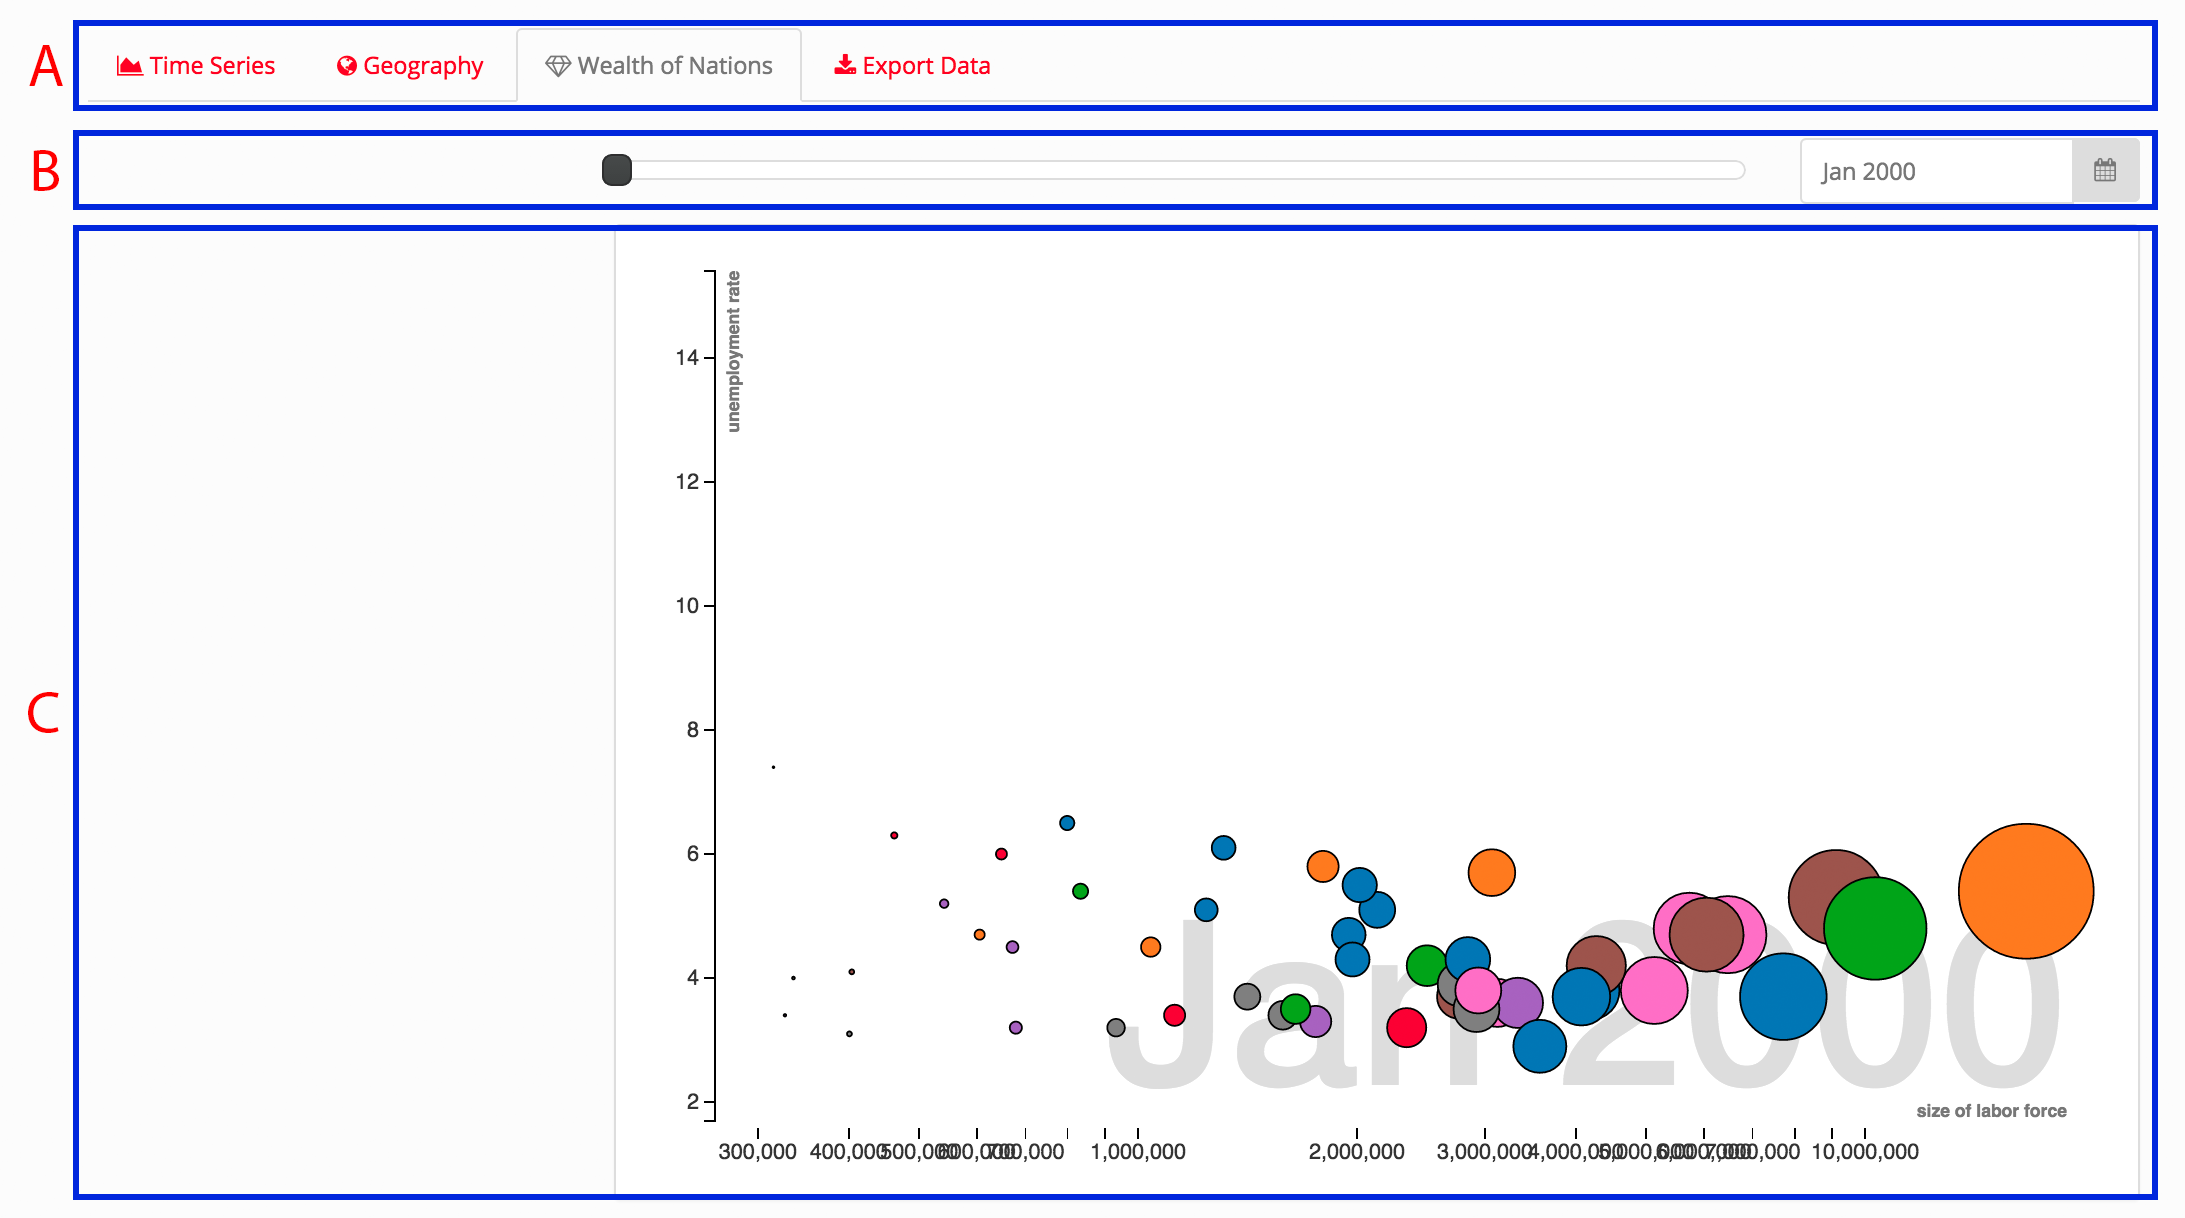
\includegraphics[width=1.75\columnwidth]{figures/wealth_new_1.png}
    \caption{A four dimensional visualization inspired by the famous ``Wealth and Health of Nations'' visualization. This visualization attempts to minimize the regional sizing of the geographic choropleth by encoding data in five dimensions: the X and Y axis representing an labor force characteristic, color representing region, and size representing the state's employment level. Finally, a slider controls the time dimension.}
    \label{fig:wealth}
\end{figure*}

Our final dashboard implements the ``Wealth and Health of Nations'' visualization that was made famous by Hans Rosling's 2006 TED Talk \cite{_wealth_????} and which demonstrates many interesting capabilities of D3. We implemented this visualization to show how multiple D3 visualizations from the gallery could easily be added to the dashboard, but also to show how different dimensions from similar data could be visualized differently. In this case, the use of a scatter plot design instead of a choropleth to describe regional information. The dashboard is broken into regions as shown in Figure~\ref{fig:wealth}.

Region C is the main part of this dashboard which contains the scatter plot, which incodes data in 5 dimensions: $x$ and $y$ axes, color, raidus, and time. The $x$-axis represents the size of labor-force and the $y$-axis represents unemployment rate. Each dot represents a state and the radius of the dot represents the employment level of that state. Each state is colored according to their economic region (e.g. northeast, midwest, west, etc). Moreover, user can select the time point of the data by moving the mouse left and right in the time region. By hovering the mouse over the plate, the name of that state will be shown. This dashboard provides a easy way of exploring insights based on two or even more different dimensions of the data for all the states simultaneously.

Region B does not appear in our original design. However, when we carried out our usability study, we found that many users complain about the difficulty to choose the time by just moving the mouse left and right on the time region, especially when the user want to fix the time point and hover on the plate to show the name of the state. In order to fix this question raised in the study, the common year slider is added to the top, consistent with other slider designs.

\subsection{Data Export}

Finally, the last dashboard implements a data exporting feature. Although this utility is not a visual analysis tool, it is meant to augment users who are using Excel or Tableau to perform their own analyses. The ingestion and wrangling of time series data is not difficult, but it is time consuming. By allowing users to directly export the data from our tool, we hope to increase the number of analyses available, and the insights that can be gained. This tool has similar controls to the dashboards whose data you can export from. Datasets are then downloaded in CSV or JSON format.

\subsection{Data Management}

Because the ingestion utility is real time and because we expect that the visual analysis dashboards will change over time, we have implemented an admin screen that gives users an at-a-glance look at the state of the system as shown in Figure~\ref{fig:admin}. We hope to convey in this page the effort it took to wrangle and gather the data, but also provide a means for interacting with the real time ingestion system. For example, an ingestion log shows when data was fetched from the BLS web site, and the magnitude of the ingestion process.

Other details include the current version of the application, and the timestamps of the updates or ingestions. The ELMR Status bar gives a quick view of any required maintenance for the system. A GREEN status indicates that the app is within a month of the last ingestion, YELLOW indicates that the app is less than six months since ingestion, and RED indicates that the app is unusable due to the amount of time since the ingestion. Database records also indicate the state and size of the database.

By creating an open utility that shows the ingestion process and the state of the database, we hope to allow users to have transparency in our analytical and systems methodology so that collaborative efforts can improve the system. Along these lines, our software is open source on Github, with links to full documentation, agile development boards, API documentation, and more all in the drop down. In the future, we hope to allow direct administration from this page, by kicking off ingestion, or editing time series directly.

\begin{figure*}[!ht]
    \centering
    \includegraphics[width=1.75\columnwidth]{figures/Admin.png}
    \caption{Illustration of Admin resources.}
    \label{fig:admin}
\end{figure*}

\section{Usability Study}

To evaluate the usability of our ELMR for analyzing the employment situation, we recruited 8 participants to carry our usability study. All these participants are male PhD students from ECE or computer science department of UMD who has no professional knowledge of economics and labor force. Our usability study contains five main parts: background introduction, training, testing by completing research-driven tasks, testing by exploring features of user interests and questionnaire. The test takes around 10~15 minutes.

\subsection{Background Introduction}
We first give a very brief introduction of our project by showing a pre-recorded video. Since none of our participants is familiar with the employment data, we also introduce the three data sets we use: CPS, CES and LAU in a little more detail.


\subsection{Training}
To train the participants how to use ELMR, we first introduce the main components of the dashboard. Then we give an example of how to draw ``Employment ratio'' and ``employment-Population ratio'' using our time series data. During the training process, we encourage the participants to think-out-loud and ask any questions they cannot understand.

\subsection{Testing by Completing Research-Driven Tasks}
After the training session, the participants are asked to work on themselves to complete 5 research driven tasks using our tool. The eight questions are as follows:
\begin{enumerate}
\item    Show the time series of unemployment rate for Asian and White people. From 2008-2010, which group of people has higher relative changes of unemployment rate.

\item    which state has the highest unemployment rate in Oct. 2011
\item    In Mar 2011, which five states has the highest size of labor force, do they also have the highest employment level
\item     Show the time series of unemployment rate for Maryland and Florida
\item     Download a data set you are interested in.
\end{enumerate}

During the test session, we will record the time the participants spend on each of these questions. We encourage the user to think through each of these questions, telling us their thoughts when they try to answer each questions.

\subsection{Exploring User Interests feature}
After answering the 5 research driven questions. The participants are asked to propose one or two questions which are interests to them about the employment status of US and explore the answer their questions using our tool. Similarly, the participants are encouraged to think-out-loud, telling us any thoughts they have during answering the questions.

\subsection{questionnaire}
After finishing answering the above questions, the participants are asked to do a questionnaire which asks the participants to give their evaluation about our tool, and how difficult it is to answer each of our research driven questions.


\subsection{Results of Usability Test}
The typical responses of subjects regarding the questions are shown in the following:


\begin{enumerate}
\item    Show the time series of unemployment rate for As and white people. From 2008-2010, which group of people has higher relative changes of unemployment rate.


All of the subjects were able to answer this question by using the time series visualization, but they complained that if the y axis are aligned or they could put different series in one chart, they could have answered this kind of questions more efficiently.

\item    which state has the highest unemployment rate in Oct. 2011


When design this question, we suppose subjects to use the geography view to find the answer. However, since the wealth of nations part also visualize the unemployment rate of states over time, one subjects used this view to find the right answer. The other 4 subjects chose the geography view. Some of them complained that when the data of two states are very similar, they could not tell which one is bigger, so they suggested that when mouse is hovering on a state, the corresponding data should be shown for easier comparison. Most of the subjects were not happy with the the way they can choose the date, they wanted a time picker to pick a specific time point, but they all liked the slide bar because it enables them to see the animated change over time. In general, they all like the heat map since it is very visually informative and appealing.


\item    In Mar 2011, which five states has the highest size of labor force, do they also have the highest employment level?

This question is the most difficult question according to the feedback of users. They all attempted to answer this question using the Wealth of Nations view, but they still could not answer it quickly due to two reasons: it is pretty hard to choose time in this view, users have to be very careful about moving their mouse; the second reason is they are not sure what the size of the bubble stands for, so some of they were not able to answer the second part of the question.


\item     Show the time series of unemployment rate for Maryland and Florida
This seems to be an easy problem for the subjects, though two of them had a little difficulty to find these two data in the drop menu in the Time Series part, they were overwhelmed by the large dataset. They thought it would be good to organize the data or choose the data in a better fashion,

\item     Download a data set you are interested in.

Subjects finished this task very quickly, and they liked this feature because in this way, they can download the data they want and use other powerful visualization tools to find more insights.

\end{enumerate}

Based on the results of the usability study, we have improved our visualization with more functions like hints and more details to help users use it. For example, in the final version of our visualization, we have added a slide bar in the wealth of nations part to help users accurately select time. To help users compare two time series, we have aligned the x-axis of the . We also added an option to select different color scale in the heat map.

%\subsection{Usability Study Settings}
%Our usability test follow the guidelines stated in class:
%\begin{itemize}

%\item We conduct the test with several users using the "thinking aloud" method of data collection
%\item We ask several research driven questions and require users to find the answers with our tool
%\item The result of our study will be bugs, features, problems, etc. to add to our tool along with their severity and priority
%\end{itemize}

\section{Related Work}

Our work captures many different facets of visual analyses as described in \cite{keim_mastering_2010} including the use of interactive dashboards, the use of a ``sense-making'' process, and the combination of user and computer analytical workflows. In particular, we attempt to create a hypothesis driven design that models human cognitive effort by combining the best characteristics of human pattern recognition and computer number crunching \cite{green_visual_2008}. We focus specifically on the cognitive pattern ``overview first, zoom and filter, details on demand'' as described in \cite{heer_interactive_2012}. This idea was taken further in \cite{heer_design_2008} to discuss collaborative interactive design, something we did not implement in our system, but hope to in the future. Collaborative interactive design allows interaction by multiple users who share visualizations and explorations to further analytical workflows.

\subsection{Employment Situation Visualization}

Visualizing employment statistics such as employment and unemployment levels and rates as well as the size of the labor force is extremely important. Although the Jobs Report does provide some simple visualizations, in \cite{leonhardt_how_2014} they are specifically analyzed to show how users can be easily misled by the report. Some work has been done in domain-specific areas. For example, \cite{ashkenas_how_2014} uses 255 spark lines on a single chart to help people specifically explore how the recession reshaped the economy. In this single visualization, each spark line represents a particular industry, and the growth or decline of the chart is encoded into the graph both by the spark line as well as by color. The size of each industry is represented along a sliding X scale. This methods, while interesting and interactive, provide only a single domain to explore, and are not updated in real time when new data is ingested.

In \cite{battista_motion_2011}, BLS researchers specifically look at how to visualize complex statistical data using motion charts - where data is encoded not just in the chart, but through movement over time. Our work uses many of these features without explicitly considering themselves motion charts since we use many dimensions besides time in our analyses. However this paper clearly shows how different analyses and time series can be combined into much simpler graphs for story telling purposes, and are good candidates for inclusion in future dashboards.

\subsection{Time Series Data Visualization}

Since the employment statistics are mostly time series data, some papers \cite{few_visualizing_2007,peng_method_2008,ashkenas_how_2014} about visualizing time series are also related to our project. \cite{few_visualizing_2007}  gives us a brief idea of which patterns of change we should pay attention to for time series data; \cite{peng_method_2008} shows how to visualize multi-dimensional time series data with different location information; and \cite{ashkenas_how_2014} focuses on visualizing the job change during the recession, which is very similar to part of what we want to visualize.


\subsection{Geography-Based Data Visualization}

For many users, they may want to visualize and compare the data for different regions or states. For example, a user may want to see how the unemployment ratio changes in the state where he or she lives. As a result, an informative visualization should give the option that users can visualize the data for different states. To achieve this function, many visualizations use a map and visualize the data by painting the map with colors, in which users can compare the regions they are interested in. For example, \cite{rodrigues_estimating_2013} invests the relationship between employment size and points-of-interest by proposing several visualization techniques to visualize this relationship in Boston metropolitan area. \cite{feldt_tailor-made_2005} creates a coordinates view that contains a Swedish map to show statistics of Sweden, and help users to explore various kinds of data that they are interested in.

Choropleths are also widely explored - and are available in a number of analytical tools. These types of charts are often criticized because they hide important data in regions that are geographically small. They also suffer from similar problems as heatmaps because color scale is vital in their creation. In \cite{brewer_mapping_1997}, the use of color in choropleths is explored to show how mortality can be better analyzed with different color schemes. Because we used both D3 \cite{bostock_d3_2011} and ColorBrewer in our work, we tried to alleviate some of these color concerns by allowing the user to select the color scale.

\section{Conclusion}

In this project we have created an interactive visual analysis tool that implements visual dashboards for human-driven insights into the BLS Employment Situation Report. Our tool aggregates over a thousand time series, ingested using the BLS API on a monthly basis and makes it available for at-a-glance insights, and visual exploration. In particular, we have created three primary dashboards: a Time Series explorer where users can compare and contrast multiple time series through a stacked overlay, a Geographic Choropleth map to investigate changes in employment according to demographics or industry at the state level, and a Wealth of Nations style dashboard that encodes multiple dimensions into a single one.

For future work, we hope to continue to augment the system and fix bugs. In particular, we want to create better interactivity with the time series explorer tool, allowing for hiding and showing time series without removing them, and doing computation on particular analyses like rate of change or finding ``spikes'' by computing the cosine angle between series. The choropleth maps could also be augmented with better details, a critique that could apply to all of our dashboards which do a decent job of ``overview'' and ``zoom and filter'' but less so on ``details on demand''. If possible we will continue to extend our work and add more visualizations in the future.

\section{Acknowledgments}

We would like to especially say thanks to Jonathan Schwabish of the Urban Institute for being our mentor, responding to emails, and giving us the idea for the project in the first place. We would also like to thank Tyrone Grandison, a Presidential Innovation Fellow at the Department of Labor for giving us guidance with using the BLS API and to Emily Liddel, also at BLS, who gave us specific information and guidance on what data sets to use. All three of our mentors helped us push the project forward when we were stalled. We'd also like to thank those folks who participated in our usability study, and who critiqued our work to help make it better. We'd also like to thank our professor Ben Shneiderman for being so enthusiastic about our project and the opportunity to present at BLS.

\balance{}

% If you want to use smaller typesetting for the reference list,
% uncomment the following line:
% \small
\bibliographystyle{acm-sigchi}
\bibliography{paper}

\newpage{}

\balance{}

\section{Credits}

The section lists the contributions of each member of the team.

\subsection{Benjamin Bengfort}

\begin{enumerate}
    \item Wrote original proposal and proposal drafts
    \item Created initial design 1
    \item Primary point of contact for mentors Jon Schwabish and Ty Grandison
    \item Created several usability study questions
    \item Implemented the data ingestion system
    \item Implemented the backend software
    \item Implemented the front end software and D3 visualizations
    \item Created presentation
    \item Presented in class and at BLS
    \item Wrote the final draft of the paper
\end{enumerate}

\subsection{Xintong Han}

\begin{enumerate}
    \item Created initial design 2
    \item Conducted usability study
    \item Produced and narrated the video
    \item Wrote the first draft of the final report
\end{enumerate}

\subsection{Assaf Magen}

\begin{enumerate}
    \item Revised the inital proposal
    \item Created initial design 1
    \item Wrote the script for the video
    \item Contributed statistical methodologies
    \item Performed data exploration and wrangling
    \item Assisted in software development tasks
\end{enumerate}

\subsection{Hao Zhou}

\begin{enumerate}
    \item Created initial design 2
    \item Created several usability study questions
    \item Conducted usability study
    \item Produced and directed the video
    \item Wrote the first draft of the final report
\end{enumerate}

\end{document}
